\chapter{Shapes and Solids}\label{ch:g2:shapes}

Flat shapes live on paper; solids fill your hands. This chapter
sorts flat shapes by counting sides and corners, tests the right
angle with a folded paper corner, and meets the first solids ---
whose faces are the flat shapes we already know.

\section{Sorting flat shapes}

\begin{definition}[Straight-sided and round]\label{def:g2:shapes:sort}
A shape whose border is made only of straight sides is a
\emph{polygon}: triangle ($3$ sides), quadrilateral ($4$ sides:
squares and rectangles are quadrilaterals), pentagon ($5$),
hexagon ($6$). A shape with a curved border, like the circle, is
\emph{not} a polygon.
\end{definition}

\begin{omfigure}
\begin{tikzpicture}[scale=0.62]
  \draw[thick, fill=omDef!12] (0,0) -- (1.8,0) -- (0.9,1.5) -- cycle;
  \node[below, font=\small] at (0.9,-0.3) {$3$ sides};
  \begin{scope}[xshift=3.2cm]
  \draw[thick, fill=omThm!12] (0,0) rectangle (1.7,1.5);
  \node[below, font=\small] at (0.85,-0.3) {$4$ sides};
  \end{scope}
  \begin{scope}[xshift=6.4cm]
  \draw[thick, fill=omMeth!12] (90:1.0) -- (162:1.0) -- (234:1.0) --
    (306:1.0) -- (18:1.0) -- cycle;
  \node[below, font=\small] at (0,-1.25) {$5$ sides};
  \end{scope}
  \begin{scope}[xshift=9.8cm]
  \draw[thick, fill=omProp!12] (0,0.75) circle (0.75);
  \node[below, font=\small] at (0,-0.35) {round};
  \end{scope}
\end{tikzpicture}

{\small Sorting by the number of sides. The number of corners always
equals the number of sides.}
\end{omfigure}

\begin{method}[Testing a right angle]\label{met:g2:shapes:rightangle}
Fold a sheet of paper twice to make a sharp corner --- that corner
is a right angle. Lay it into the corner of a shape:
\begin{enumerate}
  \item if the two sides of the shape run exactly along the folded
        corner, the angle is right;
  \item if the corner is wider or narrower, it is not right.
\end{enumerate}
A square and a rectangle have four right angles.
\end{method}

\section{Reproducing on a grid}

\begin{method}[Copying a figure]\label{met:g2:shapes:copy}
On grid paper, copy a figure vertex by vertex:
\begin{enumerate}
  \item pick a corner and mark it on the empty grid;
  \item count the squares to the next corner (``$3$ right, $2$
        up'') and mark it;
  \item join the corners in order; compare with the model.
\end{enumerate}
\end{method}

\begin{omfigure}
\begin{tikzpicture}[scale=0.5]
  \draw[gray!40] (0,0) grid (5,4);
  \draw[thick, omDef] (1,1) -- (4,1) -- (4,3) -- (2,3) -- cycle;
  \begin{scope}[xshift=7cm]
  \draw[gray!40] (0,0) grid (5,4);
  \draw[thick, omThm] (1,1) -- (4,1) -- (4,3) -- (2,3) -- cycle;
  \node[font=\footnotesize, omThm] at (2.5,0.4) {the copy};
  \end{scope}
\end{tikzpicture}

{\small A figure and its copy, made by counting squares between the
corners.}
\end{omfigure}

\section{Solids}

\begin{definition}[First solids]\label{def:g2:shapes:solids}
Solids take up space. Their flat sides are \emph{faces}:
\begin{itemize}
  \item the \emph{cube}: $6$ square faces (a die);
  \item the \emph{box} (rectangular prism): $6$ rectangle faces (a
        cereal packet);
  \item the \emph{cylinder}: two round faces and a rolled side (a
        can);
  \item the \emph{ball}: perfectly round, no flat face.
\end{itemize}
Solids and their faces return in \cref{ch:g5:solids}.
\end{definition}

\begin{omfigure}
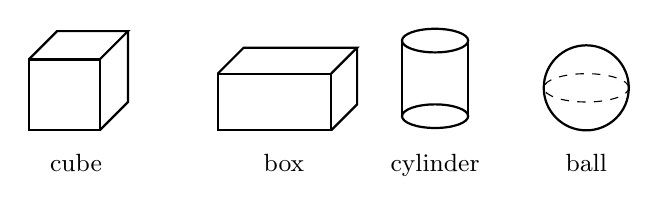
\begin{tikzpicture}[scale=0.6]
  \draw[thick] (0,0) rectangle (1.5,1.5);
  \draw[thick] (0,1.5) -- (0.6,2.1) -- (2.1,2.1) -- (1.5,1.5);
  \draw[thick] (2.1,2.1) -- (2.1,0.6) -- (1.5,0);
  \node[below, font=\small] at (1.0,-0.3) {cube};
  \begin{scope}[xshift=4.0cm]
  \draw[thick] (0,0) rectangle (2.4,1.2);
  \draw[thick] (0,1.2) -- (0.55,1.75) -- (2.95,1.75) -- (2.4,1.2);
  \draw[thick] (2.95,1.75) -- (2.95,0.55) -- (2.4,0);
  \node[below, font=\small] at (1.4,-0.3) {box};
  \end{scope}
  \begin{scope}[xshift=8.6cm]
  \draw[thick] (0,0.3) ellipse (0.7 and 0.25);
  \draw[thick] (-0.7,0.3) -- (-0.7,1.9);
  \draw[thick] (0.7,0.3) -- (0.7,1.9);
  \draw[thick] (0,1.9) ellipse (0.7 and 0.25);
  \node[below, font=\small] at (0,-0.3) {cylinder};
  \end{scope}
  \begin{scope}[xshift=11.8cm]
  \draw[thick] (0,0.9) circle (0.9);
  \draw[dashed] (0,0.9) ellipse (0.9 and 0.3);
  \node[below, font=\small] at (0,-0.3) {ball};
  \end{scope}
\end{tikzpicture}

{\small The first solids. Run a finger over a cube: you feel $6$ flat
faces and sharp edges; a ball has none.}
\end{omfigure}

\section{Exercises}

\begin{exercise}[$\star$]\label{exo:g2:shapes:1}
For each, count sides and corners and name it: a shape with $5$
sides; a shape with $3$ corners; a round shape.
\end{exercise}

\begin{exercise}[$\star$]\label{exo:g2:shapes:2}
Sort into ``polygon'' or ``not a polygon'': a square; a circle; a
triangle; a hexagon.
\end{exercise}

\begin{exercise}[$\star$]\label{exo:g2:shapes:3}
Make a right-angle tester by folding paper. Find three right angles
in the room, and one angle that is not right.
\end{exercise}

\begin{exercise}[$\star$]\label{exo:g2:shapes:4}
How many right angles has a square? A rectangle? A triangle can have
at most how many? (Try to draw one with two.)
\end{exercise}

\begin{exercise}[$\star$]\label{exo:g2:shapes:5}
On grid paper, copy a rectangle that is $4$ squares wide and $2$
tall, then a triangle with a $3$-square base.
\end{exercise}

\begin{exercise}[$\star$]\label{exo:g2:shapes:6}
Name the solid: a die; a can of soup; a football; a shoebox.
\end{exercise}

\begin{exercise}[$\star$]\label{exo:g2:shapes:7}
How many faces has a cube? What shape is each face? How many faces
has a box?
\end{exercise}

\begin{exercise}[$\star$]\label{exo:g2:shapes:8}
Which solids can roll: the cube, the box, the ball, the cylinder?
Why?
\end{exercise}

\begin{exercise}[$\star$]\label{exo:g2:shapes:9}
A shape has $6$ sides. What is it called? How many corners has it?
\end{exercise}

\begin{exercise}[$\star\star$]\label{exo:g2:shapes:10}
On grid paper, draw a house: a square for the wall
($4 \times 4$) with a triangle roof on top. How many sides and
corners has the whole outline of the house?
\end{exercise}
